\documentclass[12pt,oneside,a4paper]{report}

\usepackage[left=3cm,
			right=2.5cm,
			top=2.5cm,
			bottom=2.5cm,
			includehead,
			includefoot]{geometry}

\usepackage{setspace}
\setstretch{1,25} % 15/12 --> 1.25

%de­fines Adobe Times Ro­man as de­fault text font
\usepackage{mathptmx}
\usepackage{times} % needed for acronym package

\usepackage[hidelinks]{hyperref}

\usepackage[ngerman]{babel}
\usepackage[numbers]{natbib}
\usepackage[fixlanguage]{babelbib}
\selectbiblanguage{german}
\bibliographystyle{unsrturl}
\usepackage[T1]{fontenc}
\usepackage[utf8]{inputenc}

\AtBeginDocument{\renewcommand{\chaptername}{}}

\usepackage{enumitem}
\usepackage{tabularx}

% math packages
\usepackage{amsmath}
\usepackage{nicefrac}
\usepackage{amsthm}
\usepackage{amsbsy}
\usepackage{amssymb}
\usepackage{amsfonts}
\usepackage{MnSymbol}

% patches for latex
\usepackage{fixltx2e}

%special characters
\usepackage{amssymb}
\usepackage{upgreek,textgreek}

% acronym package
\usepackage[printonlyused, footnote]{acronym}

% breakable text in \seqsplit{}
\usepackage{seqsplit}

% \textmu
\usepackage{textcomp}

% package provides a way to compile sections of a document using the same preamble as the main document
\usepackage{subfiles}

% driver-independent color extension - used by listings,tabularx
\usepackage[usenames,dvipsnames,table,xcdraw]{xcolor}

% -- SYNTAX HIGHLIGHTING --
\usepackage{listings}
%% bash command line Syntax Highlighting
\lstdefinestyle{BASH_CMD}{ 
  columns=fullflexible,            % copy pasteable listings
  language=bash,
  basicstyle=\small\sffamily,
  basicstyle   = \small \ttfamily,
  keywordstyle = [1]\small \ttfamily,
  keywordstyle = [2]\small \ttfamily,
  commentstyle = \small \ttfamily,
  numbers=none,
  captionpos=b, 
  breaklines=true,
  numberstyle=\tiny,
  numbersep=3pt,
  frame=tlrb,
  columns=fullflexible,
  backgroundcolor=\color{white!20},
  linewidth=\linewidth,
  literate=                        % replace in code
     {Ö}{{\"O}}1
     {Ä}{{\"A}}1
     {Ü}{{\"U}}1
     {ß}{{\ss}}2
     {ü}{{\"u}}1
     {ä}{{\"a}}1
     {ö}{{\"o}}1
}
 % adds style BASH_CMD
%% Matlab Syntax Highlighting
\colorlet{keyword}{blue!100!black!80}
\colorlet{STD}{Lavender}
\colorlet{comment}{green!90!black!90}
\definecolor{mygreen}{rgb}{0,0.6,0}
\definecolor{mygray}{rgb}{0.5,0.5,0.5}
\definecolor{mymauve}{rgb}{0.58,0,0.82}


\lstdefinestyle{BASH_SCRIPT}{ 
  language     = bash,
  basicstyle   = \footnotesize \ttfamily,
  keywordstyle = [1]\color{keyword}\bfseries,
  keywordstyle = [2]\color{STD}\bfseries,
  commentstyle = \color{mygreen}\itshape,
  backgroundcolor=\color{white},   % choose the background color; you must add \usepackage{color} 
  columns=fullflexible,            % copy pasteable listings
                                   % or \usepackage{xcolor}
  basicstyle=\footnotesize,        % the size of the fonts that are used for the code
  breakatwhitespace=false,         % sets if automatic breaks should only happen at whitespace
  breaklines=true,                 % sets automatic line breaking
  captionpos=b,                    % sets the caption-position to bottom
  extendedchars=true,              % lets you use non-ASCII characters; for 8-bits encodings only,
                                   % does not work with UTF-8
  frame=single,                    % adds a frame around the code
  keepspaces=true,                 % keeps spaces in text, useful for keeping indentation of code
                                   % (possibly needs columns=flexible)
  numbers=left,                    % where to put the line-numbers; possible values are 
                                   % (none, left, right)
  numbersep=5pt,                   % how far the line-numbers are from the code
  numberstyle=\tiny\color{mygray}, % the style that is used for the line-numbers
  rulecolor=\color{black},         % if not set, the frame-color may be changed on line-breaks
                                   % within not-black text (e.g. comments (green here))
  showspaces=false,                % show spaces everywhere adding particular underscores; it
  	                               % overrides 'showstringspaces'
  showstringspaces=false,          % underline spaces within strings only
  showtabs=false,                  % show tabs within strings adding particular underscores
  stepnumber=1,                    % the step between two line-numbers. If it's 1, each line 
                                   % will be numbered
  stringstyle=\color{mymauve},     % string literal style
  tabsize=2,                       % sets default tabsize to 2 spaces
  title=\lstname,                  % set title name
  literate=                        % replace in code
     {Ö}{{\"O}}1 
     {Ä}{{\"A}}1 
     {Ü}{{\"U}}1 
     {ß}{{\ss}}2 
     {ü}{{\"u}}1 
     {ä}{{\"a}}1 
     {ö}{{\"o}}1 
     {â}{{\^{a}}}1 
     {Â}{{\^{A}}}1 
     {ç}{{\c{c}}}1 
     {Ç}{{\c{C}}}1 
     {ğ}{{\u{g}}}1 
     {Ğ}{{\u{G}}}1 
     {ı}{{\i}}1 
     {İ}{{\.{I}}}1 
     {ş}{{\c{s}}}1 
     {Ş}{{\c{S}}}1 
} % adds style BASH_SCRIPT
% Matlab Syntax Highlighting
\colorlet{keyword}{blue!100!black!80}
\colorlet{STD}{red}
\colorlet{comment}{green!90!black!90}
\definecolor{mygreen}{rgb}{0,0.6,0}
\definecolor{mygray}{rgb}{0.5,0.5,0.5}
\definecolor{mymauve}{rgb}{0.58,0,0.82}


\lstdefinestyle{LATEX}{ 
  language     = [LaTeX]{TeX},
  basicstyle   = \footnotesize \ttfamily,
  keywordstyle = [1]\color{keyword}\bfseries,
  keywordstyle = [2]\color{comment}\bfseries,
  commentstyle = \color{mygray}\itshape,
  %backgroundcolor=\color{white},   % choose the background color; you must add \usepackage{color} 
                                   % or \usepackage{xcolor}
  basicstyle=\footnotesize,        		   % the size of the fonts that are used for the code
  breakatwhitespace=false,         % sets if automatic breaks should only happen at whitespace
  columns=fullflexible,            % copy pasteable listings
  breaklines=true,                 % sets automatic line breaking
  captionpos=c,                    % sets the caption-position to bottom
  extendedchars=true,              % lets you use non-ASCII characters; for 8-bits encodings only,
                                   % does not work with UTF-8
  frame=single,                    % adds a frame around the code
  keepspaces=true,                 % keeps spaces in text, useful for keeping indentation of code
                                   % (possibly needs columns=flexible)
  numbers=left,                    % where to put the line-numbers; possible values are 
                                   % (none, left, right)
  numbersep=4pt,                   % how far the line-numbers are from the code
  numberstyle=\tiny\color{mygray}, % the style that is used for the line-numbers
  rulecolor=\color{black},         % if not set, the frame-color may be changed on line-breaks
                                   % within not-black text (e.g. comments (green here))
  showspaces=false,                % show spaces everywhere adding particular underscores; it
  	                               % overrides 'showstringspaces'
  showstringspaces=false,          % underline spaces within strings only
  showtabs=false,                  % show tabs within strings adding particular underscores
  stepnumber=1,                    % the step between two line-numbers. If it's 1, each line 
                                   % will be numbered
  stringstyle=\color{mymauve},     % string literal style
  tabsize=2,                       % sets default tabsize to 2 spaces
  title=\lstname,                  % set title name
  literate=                        % replace in code
     {Ö}{{\"O}}1 
     {Ä}{{\"A}}1 
     {Ü}{{\"U}}1 
     {ß}{{\ss}}2 
     {ü}{{\"u}}1 
     {ä}{{\"a}}1 
     {ö}{{\"o}}1 
     {â}{{\^{a}}}1 
     {Â}{{\^{A}}}1 
     {ç}{{\c{c}}}1 
     {Ç}{{\c{C}}}1 
     {ğ}{{\u{g}}}1 
     {Ğ}{{\u{G}}}1 
     {ı}{{\i}}1 
     {İ}{{\.{I}}}1 
     {ş}{{\c{s}}}1 
     {Ş}{{\c{S}}}1 
} % adds style LATEX
%% Matlab Syntax Highlighting
\colorlet{keyword}{blue!100!black!80}
\colorlet{STD}{Lavender}
\colorlet{comment}{green!90!black!90}
\definecolor{mygreen}{rgb}{0,0.6,0}
\definecolor{mygray}{rgb}{0.5,0.5,0.5}
\definecolor{mymauve}{rgb}{0.58,0,0.82}


\lstdefinestyle{MATLAB}{ 
  language     = Matlab,
  basicstyle   = \footnotesize \ttfamily,
  keywordstyle = [1]\color{keyword}\bfseries,
  keywordstyle = [2]\color{STD}\bfseries,
  commentstyle = \color{mygreen}\itshape,
  backgroundcolor=\color{white},   % choose the background color; you must add \usepackage{color} 
                                   % or \usepackage{xcolor}
  basicstyle=\footnotesize,        % the size of the fonts that are used for the code
  breakatwhitespace=false,         % sets if automatic breaks should only happen at whitespace
  columns=fullflexible,            % copy pasteable listings
  breaklines=false,                % sets automatic line breaking
  captionpos=c,                    % sets the caption-position to bottom
  extendedchars=true,              % lets you use non-ASCII characters; for 8-bits encodings only,
                                   % does not work with UTF-8
  frame=single,                    % adds a frame around the code
  keepspaces=true,                 % keeps spaces in text, useful for keeping indentation of code
                                   % (possibly needs columns=flexible)
  numbers=left,                    % where to put the line-numbers; possible values are 
                                   % (none, left, right)
  numbersep=5pt,                   % how far the line-numbers are from the code
  numberstyle=\tiny\color{mygray}, % the style that is used for the line-numbers
  rulecolor=\color{black},         % if not set, the frame-color may be changed on line-breaks
                                   % within not-black text (e.g. comments (green here))
  showspaces=false,                % show spaces everywhere adding particular underscores; it
  	                               % overrides 'showstringspaces'
  showstringspaces=false,          % underline spaces within strings only
  showtabs=false,                  % show tabs within strings adding particular underscores
  stepnumber=1,                    % the step between two line-numbers. If it's 1, each line 
                                   % will be numbered
  stringstyle=\color{mymauve},     % string literal style
  tabsize=2,                       % sets default tabsize to 2 spaces
  title=\lstname,                  % set title name
  literate=                        % replace in code
     {Ö}{{\"O}}1 
     {Ä}{{\"A}}1 
     {Ü}{{\"U}}1 
     {ß}{{\ss}}2 
     {ü}{{\"u}}1 
     {ä}{{\"a}}1 
     {ö}{{\"o}}1 
     {â}{{\^{a}}}1 
     {Â}{{\^{A}}}1 
     {ç}{{\c{c}}}1 
     {Ç}{{\c{C}}}1 
     {ğ}{{\u{g}}}1 
     {Ğ}{{\u{G}}}1 
     {ı}{{\i}}1 
     {İ}{{\.{I}}}1 
     {ş}{{\c{s}}}1 
     {Ş}{{\c{S}}}1 
} % adds style MATLAB
% Matlab Syntax Highlighting
\colorlet{keyword}{blue!100!black!80}
\colorlet{STD}{Lavender}
\colorlet{comment}{green!90!black!90}
\definecolor{mygreen}{rgb}{0,0.6,0}
\definecolor{mygray}{rgb}{0.5,0.5,0.5}
\definecolor{mymauve}{rgb}{0.58,0,0.82}


\lstdefinestyle{PYTHON}{ 
  language     = Python,
  basicstyle   = \footnotesize \ttfamily,
  keywordstyle = [1]\color{keyword}\bfseries,
  keywordstyle = [2]\color{STD}\bfseries,
  commentstyle = \color{mygreen}\itshape,
  backgroundcolor=\color{white},   % choose the background color; you must add \usepackage{color} 
                                   % or \usepackage{xcolor}
  basicstyle=\footnotesize,        % the size of the fonts that are used for the code
  columns=fullflexible,            % copy pasteable listings
  breakatwhitespace=false,         % sets if automatic breaks should only happen at whitespace
  breaklines=false,                % sets automatic line breaking
  captionpos=c,                    % sets the caption-position to bottom
  extendedchars=true,              % lets you use non-ASCII characters; for 8-bits encodings only,
                                   % does not work with UTF-8
  frame=single,                    % adds a frame around the code
  keepspaces=true,                 % keeps spaces in text, useful for keeping indentation of code
                                   % (possibly needs columns=flexible)
  numbers=left,                    % where to put the line-numbers; possible values are 
                                   % (none, left, right)
  numbersep=5pt,                   % how far the line-numbers are from the code
  numberstyle=\tiny\color{mygray}, % the style that is used for the line-numbers
  rulecolor=\color{black},         % if not set, the frame-color may be changed on line-breaks
                                   % within not-black text (e.g. comments (green here))
  showspaces=false,                % show spaces everywhere adding particular underscores; it
  	                               % overrides 'showstringspaces'
  showstringspaces=false,          % underline spaces within strings only
  showtabs=false,                  % show tabs within strings adding particular underscores
  stepnumber=1,                    % the step between two line-numbers. If it's 1, each line 
                                   % will be numbered
  stringstyle=\color{mymauve},     % string literal style
  tabsize=2,                       % sets default tabsize to 2 spaces
  title=\lstname,                  % set title name
  literate=                        % replace in code
     {Ö}{{\"O}}1 
     {Ä}{{\"A}}1 
     {Ü}{{\"U}}1 
     {ß}{{\ss}}2 
     {ü}{{\"u}}1 
     {ä}{{\"a}}1 
     {ö}{{\"o}}1 
     {â}{{\^{a}}}1 
     {Â}{{\^{A}}}1 
     {ç}{{\c{c}}}1 
     {Ç}{{\c{C}}}1 
     {ğ}{{\u{g}}}1 
     {Ğ}{{\u{G}}}1 
     {ı}{{\i}}1 
     {İ}{{\.{I}}}1 
     {ş}{{\c{s}}}1 
     {Ş}{{\c{S}}}1 
} % adds style PYTHON
%% Matlab Syntax Highlighting
\colorlet{keyword}{blue!100!black!80}
\colorlet{STD}{Lavender}
\colorlet{comment}{green!90!black!90}
\definecolor{mygreen}{rgb}{0,0.6,0}
\definecolor{mygray}{rgb}{0.5,0.5,0.5}
\definecolor{mymauve}{rgb}{0.58,0,0.82}


\lstdefinestyle{CPP}{ 
  language     = C++,
  basicstyle   = \footnotesize \ttfamily,
  keywordstyle = [1]\color{keyword}\bfseries,
  keywordstyle = [2]\color{STD}\bfseries,
  commentstyle = \color{mygreen}\itshape,
  backgroundcolor=\color{white},   % choose the background color; you must add \usepackage{color} 
                                   % or \usepackage{xcolor}
  columns=fullflexible,            % copy pasteable listings
  basicstyle=\footnotesize,        % the size of the fonts that are used for the code
  breakatwhitespace=false,         % sets if automatic breaks should only happen at whitespace
  breaklines=false,                % sets automatic line breaking
  captionpos=c,                    % sets the caption-position to bottom
  extendedchars=true,              % lets you use non-ASCII characters; for 8-bits encodings only,
                                   % does not work with UTF-8
  frame=single,                    % adds a frame around the code
  keepspaces=true,                 % keeps spaces in text, useful for keeping indentation of code
                                   % (possibly needs columns=flexible)
  numbers=left,                    % where to put the line-numbers; possible values are 
                                   % (none, left, right)
  numbersep=5pt,                   % how far the line-numbers are from the code
  numberstyle=\tiny\color{mygray}, % the style that is used for the line-numbers
  rulecolor=\color{black},         % if not set, the frame-color may be changed on line-breaks
                                   % within not-black text (e.g. comments (green here))
  showspaces=false,                % show spaces everywhere adding particular underscores; it
  	                               % overrides 'showstringspaces'
  showstringspaces=false,          % underline spaces within strings only
  showtabs=false,                  % show tabs within strings adding particular underscores
  stepnumber=1,                    % the step between two line-numbers. If it's 1, each line 
                                   % will be numbered
  stringstyle=\color{mymauve},     % string literal style
  tabsize=2,                       % sets default tabsize to 2 spaces
  title=\lstname,                  % set title name
  literate=                        % replace in code
     {Ö}{{\"O}}1 
     {Ä}{{\"A}}1 
     {Ü}{{\"U}}1 
     {ß}{{\ss}}2 
     {ü}{{\"u}}1 
     {ä}{{\"a}}1 
     {ö}{{\"o}}1 
     {â}{{\^{a}}}1 
     {Â}{{\^{A}}}1 
     {ç}{{\c{c}}}1 
     {Ç}{{\c{C}}}1 
     {ğ}{{\u{g}}}1 
     {Ğ}{{\u{G}}}1 
     {ı}{{\i}}1 
     {İ}{{\.{I}}}1 
     {ş}{{\c{s}}}1 
     {Ş}{{\c{S}}}1 
} % adds style CPP
%% Matlab Syntax Highlighting
\colorlet{keyword}{blue!100!black!80}
\colorlet{STD}{Lavender}
\colorlet{comment}{green!90!black!90}
\definecolor{mygreen}{rgb}{0,0.6,0}
\definecolor{mygray}{rgb}{0.5,0.5,0.5}
\definecolor{mymauve}{rgb}{0.58,0,0.82}


\lstdefinestyle{C}{ 
  language     = C,
  basicstyle   = \footnotesize \ttfamily,
  keywordstyle = [1]\color{keyword}\bfseries,
  keywordstyle = [2]\color{STD}\bfseries,
  commentstyle = \color{mygreen}\itshape,
  backgroundcolor=\color{white},   % choose the background color; you must add \usepackage{color} 
  columns=fullflexible,            % copy pasteable listings
                                   % or \usepackage{xcolor}
  basicstyle=\footnotesize,        % the size of the fonts that are used for the code
  breakatwhitespace=false,         % sets if automatic breaks should only happen at whitespace
  breaklines=false,                % sets automatic line breaking
  captionpos=c,                    % sets the caption-position to bottom
  extendedchars=true,              % lets you use non-ASCII characters; for 8-bits encodings only,
                                   % does not work with UTF-8
  frame=single,                    % adds a frame around the code
  keepspaces=true,                 % keeps spaces in text, useful for keeping indentation of code
                                   % (possibly needs columns=flexible)
  numbers=left,                    % where to put the line-numbers; possible values are 
                                   % (none, left, right)
  numbersep=5pt,                   % how far the line-numbers are from the code
  numberstyle=\tiny\color{mygray}, % the style that is used for the line-numbers
  rulecolor=\color{black},         % if not set, the frame-color may be changed on line-breaks
                                   % within not-black text (e.g. comments (green here))
  showspaces=false,                % show spaces everywhere adding particular underscores; it
  	                               % overrides 'showstringspaces'
  showstringspaces=false,          % underline spaces within strings only
  showtabs=false,                  % show tabs within strings adding particular underscores
  stepnumber=1,                    % the step between two line-numbers. If it's 1, each line 
                                   % will be numbered
  stringstyle=\color{mymauve},     % string literal style
  tabsize=2,                       % sets default tabsize to 2 spaces
  title=\lstname,                  % set title name
  literate=                        % replace in code
     {Ö}{{\"O}}1 
     {Ä}{{\"A}}1 
     {Ü}{{\"U}}1 
     {ß}{{\ss}}2 
     {ü}{{\"u}}1 
     {ä}{{\"a}}1 
     {ö}{{\"o}}1 
     {â}{{\^{a}}}1 
     {Â}{{\^{A}}}1 
     {ç}{{\c{c}}}1 
     {Ç}{{\c{C}}}1 
     {ğ}{{\u{g}}}1 
     {Ğ}{{\u{G}}}1 
     {ı}{{\i}}1 
     {İ}{{\.{I}}}1 
     {ş}{{\c{s}}}1 
     {Ş}{{\c{S}}}1 
} % adds style C
%% JSON Syntax Highlighting
\colorlet{keyword}{blue!100!black!80}
\colorlet{STD}{Lavender}
\colorlet{comment}{green!90!black!90}
\definecolor{mygreen}{rgb}{0,0.6,0}
\definecolor{mygray}{rgb}{0.5,0.5,0.5}
\definecolor{mymauve}{rgb}{0.58,0,0.82}

\newcommand\JSONnumbervaluestyle{\color{blue}}
\newcommand\JSONstringvaluestyle{\color{red}}

\newif\ifcolonfoundonthisline

\makeatletter

\lstdefinelanguage{json}
{
  showstringspaces    = false,
  keywords            = {false,true},
  alsoletter          = 0123456789.,
  morestring          = [s]{"}{"},
  morestring          = [s]{'}{'},
  stringstyle         = \ifcolonfoundonthisline\JSONstringvaluestyle\fi,
  MoreSelectCharTable =%
    \lst@DefSaveDef{`:}\colon@json{\processColon@json},
  basicstyle          = \ttfamily,
  keywordstyle        = \ttfamily\bfseries,
}

% flip the switch if a colon is found in Pmode
\newcommand\processColon@json{
  \colon@json%
  \ifnum\lst@mode=\lst@Pmode%
    \global\colonfoundonthislinetrue%
  \fi
}

\lst@AddToHook{Output}{%
  \ifcolonfoundonthisline%
    \ifnum\lst@mode=\lst@Pmode%
      \def\lst@thestyle{\JSONnumbervaluestyle}%
    \fi
  \fi
  %override by keyword style if a keyword is detected!
  \lsthk@DetectKeywords% 
}

% reset the switch at the end of line
\lst@AddToHook{EOL}%
  {\global\colonfoundonthislinefalse}

\makeatother



\lstdefinestyle{JSON}{ 
  language     = json,
  basicstyle   = \footnotesize \ttfamily,
  keywordstyle = [1]\color{keyword}\bfseries,
  keywordstyle = [2]\color{STD}\bfseries,
  commentstyle = \color{mygreen}\itshape,
  backgroundcolor=\color{white},   % choose the background color; you must add \usepackage{color} 
                                   % or \usepackage{xcolor}
  basicstyle=\footnotesize,        % the size of the fonts that are used for the code
  columns=fullflexible,            % copy pasteable listings
  breakatwhitespace=false,         % sets if automatic breaks should only happen at whitespace
  breaklines=false,                % sets automatic line breaking
  captionpos=c,                    % sets the caption-position to bottom
  extendedchars=true,              % lets you use non-ASCII characters; for 8-bits encodings only,
                                   % does not work with UTF-8
  frame=single,                    % adds a frame around the code
  keepspaces=true,                 % keeps spaces in text, useful for keeping indentation of code
                                   % (possibly needs columns=flexible)
  numbers=left,                    % where to put the line-numbers; possible values are 
                                   % (none, left, right)
  numbersep=5pt,                   % how far the line-numbers are from the code
  numberstyle=\tiny\color{mygray}, % the style that is used for the line-numbers
  rulecolor=\color{black},         % if not set, the frame-color may be changed on line-breaks
                                   % within not-black text (e.g. comments (green here))
  showspaces=false,                % show spaces everywhere adding particular underscores; it
  	                               % overrides 'showstringspaces'
  showstringspaces=false,          % underline spaces within strings only
  showtabs=false,                  % show tabs within strings adding particular underscores
  stepnumber=1,                    % the step between two line-numbers. If it's 1, each line 
                                   % will be numbered
  stringstyle=\color{mymauve},     % string literal style
  tabsize=2,                       % sets default tabsize to 2 spaces
  title=\lstname,                  % set title name
  literate=                        % replace in code
     {Ö}{{\"O}}1
     {Ä}{{\"A}}1
     {Ü}{{\"U}}1
     {ß}{{\ss}}2
     {ü}{{\"u}}1
     {ä}{{\"a}}1
     {ö}{{\"o}}1
} % adds style JSON

% HEADLINE CFG
\usepackage{fancyhdr} % Headers and footers
\usepackage{lastpage}
\usepackage{nopageno}
\setlength{\headheight}{1.5cm}
\pagestyle{fancy} % All pages have headers and footers
\fancyhead{} % Blank out the default header
\fancyfoot{} % Blank out the default footer
\fancyhead[L]{}
\fancyhead[C]{}
\fancyhead[R]{}
\fancyfoot[L]{}
\fancyfoot[C]{\thepage}
\fancyfoot[R]{}
% override plain page style for \part, \chapter or
% \maketitle, which implicit specifies plain page style
\fancypagestyle{plain} 
{
	\fancyhead[L]{}
	\fancyhead[C]{}
	\fancyhead[R]{}
	\fancyfoot[L]{}
	\fancyfoot[C]{\thepage}
	\fancyfoot[R]{}
}
% set list pagestyle
\fancypagestyle{lists} 
{
	\fancyhead[L]{}
	\fancyhead[C]{}
	\fancyhead[R]{}
	\fancyfoot[L]{}
	\fancyfoot[C]{\thepage}
	\fancyfoot[R]{}
}

\renewcommand{\chaptermark}[1]{\markright{#1}{}}
\renewcommand{\sectionmark}[1]{\markright{#1}{}}
\renewcommand{\headrulewidth}{0pt}
\renewcommand{\footrulewidth}{0pt}

\usepackage{verbatim}
\usepackage{graphicx}
\usepackage{epstopdf}

% floating prevention packages
\usepackage{float}    % used with [H] positioning parameter
\usepackage{placeins} % \FloatBarrier

% tikz packages
\usepackage{tikz}
\usepackage{caption}
\usepackage[list=true,listformat=simple]{subcaption}
\usepackage{standalone}
\usepackage{pgfplots}

% include only specified tex files - uncommend unneeded
\includeonly{preface/cover,
             preface/abstract,
             preface/tableofcontents,
             preface/listoffigures,
             preface/listoftables,
             preface/lstlistoflistings,
             appendix/bibliography}

\newcommand{\strLecture}{Signale, Systeme und Sensoren}
\newcommand{\strDate}{\today}
\newcommand{\strAuthorA}{}
\newcommand{\strAuthorB}{}
\newcommand{\strAuthorAEmail}{}
\newcommand{\strAuthorBEmail}{}
% Versuchsbeschreibung
\newcommand{\strTopic}{Kalibrierung und Einsatz eines Infrarot-Entfernungsmessers}
\newcommand{\strAbstract}{
	Der Versuch nutzt die in der Vorlesung gezeigten Techniken der Kalibrierung, Fehleranalyse und Fehlerrechnung um einen Distanzsensor als Entfernungmesser nutzbar zu machen.
	
	Dieser Sensor nutzt das Triangulationsprinzip zur Bestimmung von Distanzen. Hierfür wird mittels Infrarot ein Lichtstrahl ausgesendet und der Winkel der Reflexion gemessen.

	Unser Sensor liefert eine anti-proportionale Spannung bei steigender Entfernung. Der mögliche Messbereich erstreckt sich laut Datenblatt von 10 cm bis 80 cm Entfernung zum Sensor.
}
% hyperref customization
\hypersetup{
	pdftitle    ={\strTopic}, % title
	pdfsubject	={\strLecture}, % subject of the document
	pdfauthor	={\strAuthorA, \strAuthorB}, % author
	pdfkeywords	={}, % list of keywords
	pdfcreator	={}, % creator of the document
	pdfproducer	={}, % producer of the document
	colorlinks=false, % false: boxed links; true: colored links
	linkcolor=red, % color of internal links (change box color with linkbordercolor)
    citecolor=green, % color of links to bibliography
    filecolor=magenta, % color of file links
    urlcolor=cyan, % color of external links
	bookmarks=true, % show bookmarks bar?
	unicode=true, % non-Latin characters in Acrobat’s bookmarks
	pdftoolbar=true, % show Acrobat’s toolbar?
	pdfmenubar=true, % show Acrobat’s menu?
    pdffitwindow=false, % window fit to page when opened
	pdfnewwindow=true % links in new PDF window
}

\begin{document}
\pagenumbering{Roman}

%\setcounter{section}{0}

\begin{titlepage}

\vspace*{-3.5cm}

\begin{flushleft}
\hspace*{-1cm} 
\includegraphics[width=15.7cm]{preface/htwg-logo}
\end{flushleft}

\vspace{1cm}

\begin{center}
	\large{
		\textbf{\strLecture} \\[2cm]
	}
	\Huge{
		\textbf{\strTopic} \\[2cm]
	}
	\Large{
		\textbf{\strAuthorA, \strAuthorB}} \\[3cm]
		%\textbf{\strAuthorA, \strAuthorB, \strAuthorC}} \\[3cm]
	\large{
		\textbf{} \\[2.3cm]
	}
	
	\large{
		\textbf{Konstanz, \strDate}
	}
\end{center}

\end{titlepage}
\thispagestyle{empty}




\begin{center}
{\Large \textbf{Zusammenfassung (Abstract)}}
\end{center}

\bigskip

\begin{center}
	\begin{tabular}{p{2.8cm}p{5cm}p{5cm}}
		Thema: & \multicolumn{2}{p{10cm}}{\raggedright\strTopic} \\
		 & & \\
		Autoren: & \strAuthorA & \href{mailto:\strAuthorAEmail}{\strAuthorAEmail} \\
		 & \strAuthorB & \href{mailto:\strAuthorBEmail}{\strAuthorBEmail} \\
		 & & \\
		Betreuer: & Prof. Dr. Matthias O. Franz & \href{mailto:mfranz@htwg-konstanz.de}{mfranz@htwg-konstanz.de} \\
		 &  Jürgen Keppler & \href{mailto:juergen.keppler@htwg-konstanz.de}{juergen.keppler@htwg-konstanz.de} \\
		 &  Martin Miller & \href{mailto:martin.miller@htwg-konstanz.de}{martin.miller@htwg-konstanz.de} \\
	\end{tabular}
\end{center}

\bigskip

\noindent
\strAbstract

\thispagestyle{lists}



\clearpage

\pagestyle{preface}
%
% TABLE OF CONTENTS
%
\tableofcontents
\newpage

%
% Abbildungsverzeichnis
%
\phantomsection
\addcontentsline{toc}{chapter}{Abbildungsverzeichnis}
\listoffigures
\thispagestyle{preface}
\newpage
\clearpage
%
% Tabellenverzeichnis
%
\phantomsection
\addcontentsline{toc}{chapter}{Tabellenverzeichnis}
\listoftables
\thispagestyle{lists}
\newpage
%
% Listingverzeichnis
%
\phantomsection
\renewcommand\lstlistingname{Listing}
\renewcommand\lstlistlistingname{Listingverzeichnis}
\lstlistoflistings
\addcontentsline{toc}{chapter}{Listingverzeichnis}
\thispagestyle{lists}
\newpage


\pagenumbering{arabic}
\setcounter{page}{1}

\chapter{Einleitung}
\label{chap:EINL}
Dieser Versuch beschäftigt sich mit der Kalibrierung eines Distanzsensors der Firma Sharp (GP2Y0A21YK0F, siehe Datenblatt in Moodle).

Zur Kalibrierung des Distanzsensors werden 20 Messungen durchgeführt. Bei diesen Messungen wird in Abhängigkeit der Entfernung eines Objektes zum Sensor die Ausgangsspannung und die Schwankung der Ausgangsspannung ($\vartriangle$ U) aufgezeichnet. Diese Werte werden zusätzlich zur automatischen digitalen Erfassung durch ein Python-Skript auch manuell notiert.

Mit den per Python-Skript automatisch digital erfassten Messwerten werden diese anschließend auf ihre Standardabweichung sowie ihren Durchschnitt ausgewertet.

Im folgenden werden die am Computer digital erfassten Messwerte per Python-Skript weiterverarbeitet um mittels der in der Vorlesung besprochenen Verfahren eine Ausgleichsfunktion zu bestimmen. Dies geschieht nach dem Verfahren der Linearen Regression.

Diese Ausgleichsfunktion kann nun zur direkten Umrechnung von Ausgangsspannungswerten des Distanzsensors in eine Distanz des Objektes das sich vor diesem Distanzsensor befindet genutzt werden.

Anschließend wird mit dem Sensor die Länge und Breite eines A4-Blatts vermessen werden. Anhand der zuvor berechneten Ausgleichsfunktion kann nun die Länge und Breite eines DIN A-4 Blattes berechnet werden.
Mit diesen Längen lässt sich anschließend die Fläche des DIN-4 Blattes bestimmen.
Um die Genauigkeit dieser Fläche zu bestimmen wird eine Fehlerrechnung anhand der in Vorlesung besprochenen Verfahren durchgeführt.


\chapter{Versuch 1}
\label{chap:VERSUCH_1}

\section{Fragestellung, Messprinzip, Aufbau, Messmittel}
\label{chap:VERSUCH_1_FRAGESTELLUNG}
In Versuch 1 [\ref{chap:VERSUCH_1}] soll die Kennlinie des Sensors mithilfe mehrerer Messungen an gleichmäßigen Abständen zwischen 10 cm und 70 cm ermittelt werden. Die Messungen sollen sowohl automatisch mittels eines Python-Skripts, sowie von Hand erfasst werden.

Für den Versuchsaufbau wird der Distanzsensor GP2Y0A21YK0F der Firma Sharp an eine Spannungsquelle von 5 V Gleichspannung angeschlossen. Zusätzlich wird der Distanzsensor am Anschluss für den Signalausgang, sowie am Ground-Anschluss mit einem Oszilloskop verbunden. Vor dem Sensor wird eine weiße Holzplatte in einem festgelegten Abstand aufgestellt. Das Oszilloskop wird über einen USB-Anschluss mit einem Laborcomputer verbunden, um dort eine automatische Erfassung der Messwerte vornehmen zu können.

Es werden 20 Messungen mit verschiedenen Distanzen vorgenommen. Es wird mit 10 cm Abstand vom Gehäuseende des Sensors zur Holzplatte begonnen. Bei jeder Messung wird der Abstand zwischen Sensor und Platte in gleichmäßigen Schritten vergrößert, bis er bei der 20. Messung 70 cm beträgt. Zur Ausrichtung der Holzplatte zum Sensor wird ein Meterstab verwendet.

Die Messwerte werden auf zwei Arten erfasst. Zum einen werden die Messwerte vom Display des Oszilloskops abgelesen und von Hand notiert. Zum anderen werden die Werte automatisch über das vom Tutor bereitgestellte Python-Srkipt [\ref*{chap:APPENDIX_SOURCECODE_MEASURE}] erfasst. Hierzu kommt das Python-Paket TekTDS2000 zum Einsatz.

\section{Messwerte}
\label{chap:VERSUCH_1_MESSWERTE}
Tabelle [\ref{chap:VERSUCH_1_MESSWERTE}] zeigt die von Hand notierten sowie die per Skript erfassten Messwerte

\begin{table}[H]
	\centering\small
	\begin{tabular}{|c|c|c|c|c|}
		\hline
		Abstand & Spannung & $\vartriangle$ U & Spannung (Python) & $\vartriangle$ U (Python) \\
		\hline
		10.0 cm & 1.30 V & .24 V & 1.287413333333333298e+00 & 2.000000000000001776e-01 \\
		\hline
		13.1 cm & 1.13 V & .24 V & 1.127840000000000176e+00 & 2.399999999999999911e-01 \\
		\hline
		16.3 cm & .99 V & .23 V & 9.969333333333334490e-01 & 2.399999999999998801e-01 \\
		\hline
		19.5 cm & .88 V & .22 V & 8.813866666666666516e-01 & 1.999999999999999556e-01 \\
		\hline
		22.6 cm & .80 V & .22 V & 7.999733333333332030e-01 & 2.399999999999999911e-01 \\
		\hline
		25.8 cm & .73 V & .24 V & 7.225866666666665994e-01 & 2.399999999999999911e-01 \\
		\hline
		28.9 cm & .68 V & .21 V & 6.640266666666665429e-01 & 2.399999999999999911e-01 \\
		\hline
		32.1 cm & .62 V & .22 V & 6.152266666666665884e-01 & 2.399999999999999911e-01 \\
		\hline
		35.3 cm & .56 V & .24 V & 5.532533333333333747e-01 & 2.000000000000000111e-01 \\
		\hline
		38.4 cm & .54 V & .23 V & 5.440533333333333887e-01 & 3.600000000000000422e-01 \\
		\hline
		41.6 cm & .50 V & .21 V & 5.038400000000000656e-01 & 1.999999999999999556e-01 \\
		\hline
		44.7 cm & .47 V & .24 V & 4.617066666666667096e-01 & 2.800000000000000266e-01 \\
		\hline
		47.9 cm & .44 V & .22 V & 4.430933333333333946e-01 & 3.200000000000000067e-01 \\
		\hline
		51.1 cm & .40 V & .22 V & 4.053333333333333233e-01 & 2.399999999999999911e-01 \\
		\hline
		54.2 cm & .39 V & .22 V & 3.870399999999999396e-01 & 1.999999999999999556e-01 \\
		\hline
		57.4 cm & .37 V & .23 V & 3.642933333333333024e-01 & 2.399999999999999911e-01 \\
		\hline
		60.5 cm & .35 V & .23 V & 3.438399999999999235e-01 & 3.599999999999999867e-01 \\
		\hline
		63.7 cm & .33 V & .22 V & 3.235733333333332684e-01 & 3.599999999999999867e-01 \\
		\hline
		66.4 cm & .29 V & .24 V & 3.034399999999999875e-01 & 3.999999999999999667e-01 \\
		\hline
		70.0 cm & .28 V & .22 V & 2.818933333333333291e-01 & 2.000000000000000111e-01 \\
		\hline
	\end{tabular}
	\caption{Messwerte Kalibrierung}
	\label{fig:VERSUCH_1_MESSWERTE_TABELLE}
\end{table}

\section{Auswertung}
\label{chap:VERSUCH_1_AUSWERTUNG}
Zur Veranschaulichung der Messung sind die per Python-Skript erfassten Messwerte in der Abbildung \ref{fig:VERSUCH_1_AUSWERTUNG_PLOT} dargestellt. Dieser Plot wurde mit dem Python-Skript \ref{chap:APPENDIX_SOURCECODE_PLOT} erstellt.

\begin{figure}[H]
	\centering\small
	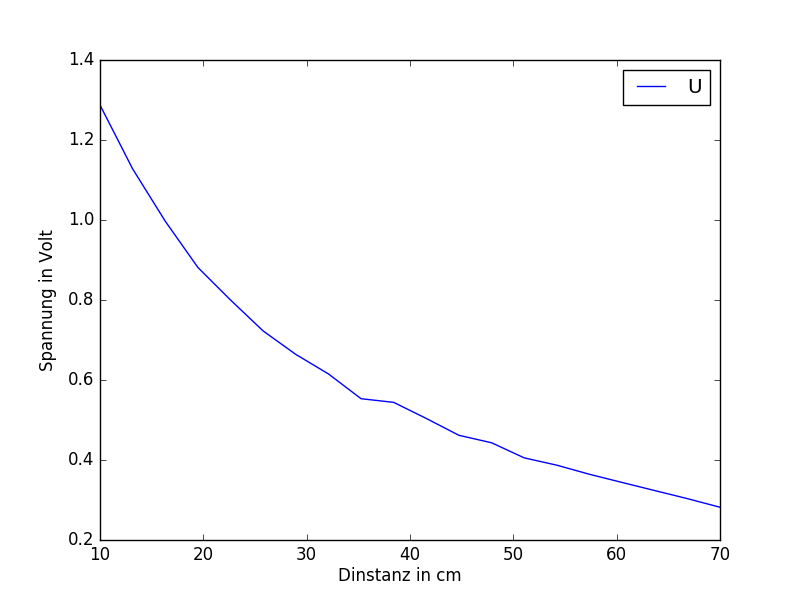
\includegraphics[width=\textwidth]{media/plot_messungen_avg.png}
	\caption{Plot Messungen}
	\label{fig:VERSUCH_1_AUSWERTUNG_PLOT}
\end{figure}

\section{Interpretation}
\label{chap:VERSUCH_1_INTERPRETATION}
Nach der Auswertung der Messwerte ist zu erkennen das sich die Ausgangsspannung anti-proportional zur Distanz der Objekte vor dem Distanzsensor verhält.

Die manuell notierten Ergebnisse der Ausgangsspannung kommen sehr nahe an die digital erstellte Messung.

Allerdings weichen die Werte der Standardabweichung $\vartriangle$ U von manueller Erhebung und digitaler Messung stark ab. Dies lässt sich darauf zurückführen das der digitale Messung 1.500 Einzelmessungen zugrunde liegen welche gemittelt sehr genau sind im Gegensatz zur manuellen Erhebung bei der einzelne Ausreißer den Wert stark beeinflussen können.


\chapter{Versuch 2}
\label{chap:VERSUCH_2}

\section{Fragestellung, Messprinzip, Aufbau, Messmittel}
\label{chap:VERSUCH_2_FRAGESTELLUNG}
Mit den in Versuch 1 [\ref{chap:VERSUCH_1}] gemessenen Werten wird nun mittels eines Regressionsverfahrens eine Funktion bestimmt mit deren Hilfe es möglich ist anhand der am Distanzsensor gemessenen Ausgangsspannung den Abstand eines Objektes zum Sensor zu bestimmen.

Für die Bestimmung dieser Funktion nutzen wir das in der Vorlesung besprochene Verfahren der linearen Regression. Allerdings lässt sich dieses Verfahren nur bei einer linearen Kennlinie anwenden, welche bei unserem Sensor nicht vorliegt (vergl. Kennlinie in Versuch 1 - Messwerte [\ref{chap:VERSUCH_1_MESSWERTE}]). Um das Verfahren trotzdem nutzen zu können werden mittels des im Aufgabenblatt gezeigten Lösungsansatzes - der Logarithmierung von Distanz und Spannung - aus den Werten in der Messwerttabelle [\ref{fig:VERSUCH_1_MESSWERTE_TABELLE}] für die lineare Regression geeignete Werte berechnet.

Als Resultat der linearen Regression erhalten wir den Gradienten \(a\), sowie das Offset \(b\). Setzt man diese Parameter in die Funktion \(y = e^b * x^a\) ein erhält man die Kennlinie des Distanzsensors. \(x\) ist hierbei die am Sensor gemessene Spannung.

\section{Messwerte}
\label{chap:VERSUCH_2_MESSWERTE}
Mit dem Python-Skript [\ref{chap:APPENDIX_SOURCECODE_LINEARE_REGRESSION}] werden die Messwerte [\ref{chap:VERSUCH_1_MESSWERTE}] aus Versuch 1 \ref{chap:VERSUCH_1} logarithmiert und in der Tabelle [\ref{fig:VERSUCH_2_MESSWERTE_TABELLE}] sowie dem Plot [\ref{fig:VERSUCH_2_MESSWERTE_PLOT}] dargestellt.

\begin{table}[H]
	\centering\small
	\begin{tabular}{|c|c|}
		\hline
		log(Distanz) & log(Spannung) \\
		\hline
		2.30258509299 & 0.252635037374 \\
		\hline
		2.5770219387 & 0.120304299043 \\
		\hline
		2.79213331831 & -0.00307137852449 \\
		\hline
		2.96906402647 & -0.126258854137 \\
		\hline
		3.11934622952 & -0.223176885203 \\
		\hline
		3.24996641194 & -0.324917912326 \\
		\hline
		3.36547929906 & -0.40943296967 \\
		\hline
		3.469019978 & -0.485764515393 \\
		\hline
		3.56283873322 & -0.591939275065 \\
		\hline
		3.64860555498 & -0.608707997716 \\
		\hline
		3.72759396629 & -0.685496521629 \\
		\hline
		3.80079737032 & -0.772825510183 \\
		\hline
		3.86900562034 & -0.813974846403 \\
		\hline
		3.93285709233 & -0.903045505124 \\
		\hline
		3.99287510206 & -0.94922723212 \\
		\hline
		4.04949399606 & -1.00979587507 \\
		\hline
		4.10307824219 & -1.06757884609 \\
		\hline
		4.15393665942 & -1.12832950346 \\
		\hline
		4.20233320029 & -1.1925713816 \\
		\hline
		4.24849524205 & -1.26622653019 \\
		\hline
	\end{tabular}
	\caption{Messwerte nach Logarithmierung}
	\label{fig:VERSUCH_2_MESSWERTE_TABELLE}
\end{table}

\begin{figure}[H]
	\centering\small
	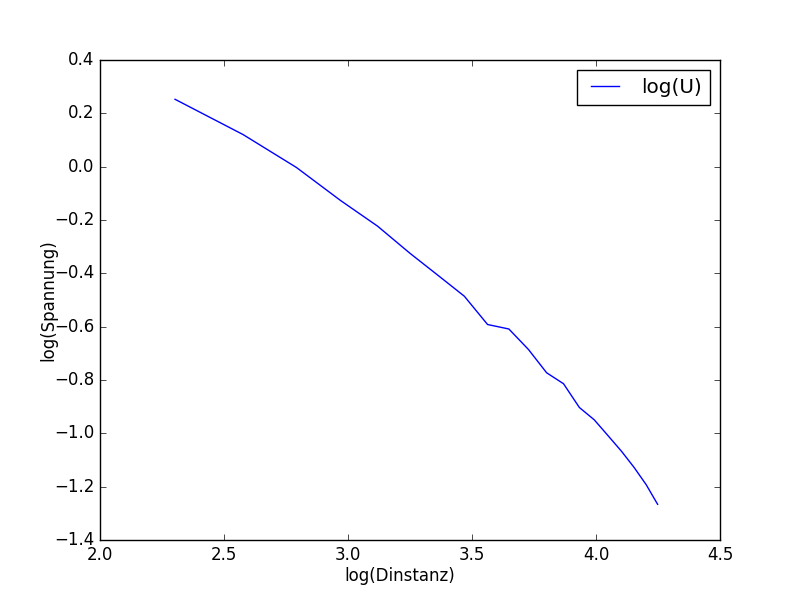
\includegraphics[width=\textwidth]{media/plot_messungen_log.png}
	\caption{Plot der Messwerte nach Logarithmierung}
	\label{fig:VERSUCH_2_MESSWERTE_PLOT}
\end{figure}

\section{Auswertung}
\label{chap:VERSUCH_2_AUSWERTUNG}
Anhand der logarithmierten Werte kann nun der Gradient berechnet werden. Diesen erhält man, wenn man die in Tabelle [\ref{fig:VERSUCH_2_MESSWERTE_TABELLE}] gezeigten Werte in die Formel \(a = \frac{\sum_{i=1}^{n}{(x_i - \overline{x}) \cdot (y_i - \overline{y})}}{\sum_{i=1}^{n}{(x_i - \overline{x}^2)}}\) einsetzt.

Mithilfe des Gradienten der logarithmierten Messwerte lässt sich über die Formel \(b = \overline{y} - a \cdot \overline{x}\) der Offset berechnen.

Dies führt zu den Werten

\(a = -1.25018776118\)

und

\(b = 2.79487428118\)

Die Kennlinie erhält man, in dem man die doppelte Logarithmierung \(exp(a \cdot \ln x + b)\) umkehrt. Daraus resultiert die Kennlinie [\ref{fig:VERSUCH_2_AUSWERTUNG_KENNLINIE}].

\begin{figure}[H]
	\centering\small
	\(y = e^{2.79487428118} \cdot x^{-1.25018776118}\)
	\caption{Kennlinie}
	\label{fig:VERSUCH_2_AUSWERTUNG_KENNLINIE}
\end{figure}

\begin{figure}[H]
	\centering\small
	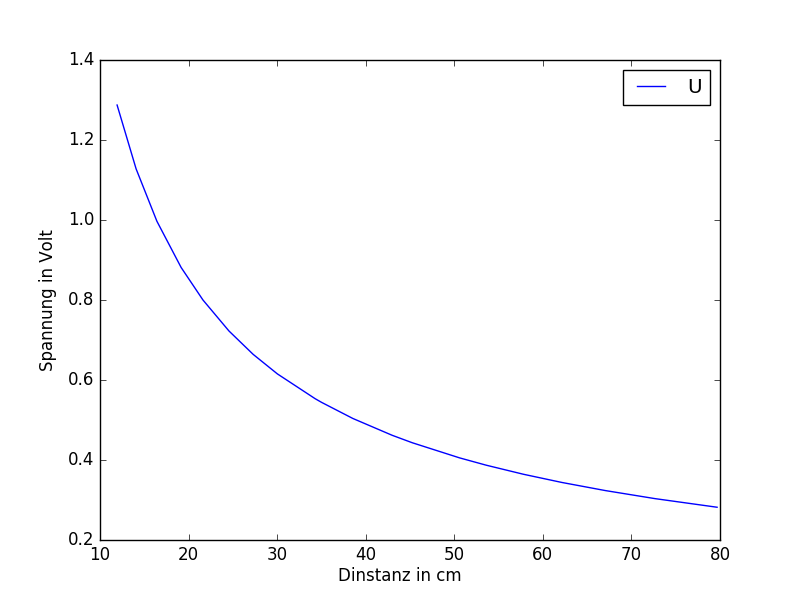
\includegraphics[width=\textwidth]{media/plot_messungen_funktion.png}
	\caption{Plot nach Linearer Regression}
	\label{fig:VERSUCH_2_AUSWERTUNG_PLOT}
\end{figure}

Bei \(x\) handelt es sich hier um die gemessene Spannung und bei \(y\) um den gemessenen Abstand.

\section{Interpretation}
\label{chap:VERSUCH_2_INTERPRETATION}
Die Grafiken [\ref{fig:VERSUCH_1_AUSWERTUNG_PLOT}] und [\ref{fig:VERSUCH_2_AUSWERTUNG_PLOT}] zeigen die gemessenen Spannungs-/Entfernungswerte, sowie die berechnete Kennlinie. Daran, dass die Kennlinie und die gemessenen Werte sehr nahe beieinander liegen, sieht man, dass das Verfahren zur Ermittlung einer nicht linearen Kennlinie mithilfe der linearen Regression mit logarithmierten Werten funktioniert.

Da jedoch nur jeweils eine Messung für die Eingangswerte vorgenommen wurde, ist der Messfehler für die Werte, aus denen die Kennlinie berechnet wurde relativ hoch. Diese Messfehler wurden in die Kennlinie eingerechnet, sodass jede Messung anhand der Kennlinie zu einem relativ hohen systematischen Fehler führt.


\chapter{Versuch 3}
\label{chap:VERSUCH_3}

\section{Fragestellung, Messprinzip, Aufbau, Messmittel}
\label{chap:VERSUCH_3_FRAGESTELLUNG}

Anschließend wird ein DIN A4-Blatt mit dem Sensor vermessen und der Flächeninhalt des Blattes anhand der Kennlinie berechnet.

\section{Messwerte}
\label{chap:VERSUCH_3_MESSWERTE}

Die Vermessung des A4-Blatts wurde mithilfe des Skripts \ref{chap:APPENDIX_SOURCECODE_MEASURE_PAPER} durchgeführt. Die resultierenden Messwerte befinden sich in Tabelle \ref{fig:VERSUCH_3_MESSWERTE_TABELLE}.

\begin{table}[H]
	\centering\small
	\begin{tabular}{|c|c|c|}
		\hline
		Abstand & Spannung & $\vartriangle$ U \\
		\hline
		21.0 cm & .91 V & .24 V \\
		\hline
		29.7 cm & .70 V & .24 V \\
		\hline
	\end{tabular}
	\caption{Messwerte A4-Blatt}
	\label{fig:VERSUCH_3_MESSWERTE_TABELLE}
\end{table}

\section{Auswertung}
\label{chap:VERSUCH_3_AUSWERTUNG}

Durch die Kennlinie \ref{fig:VERSUCH_2_AUSWERTUNG_KENNLINIE} lassen sich die Maße des DIN A 4 Blattes nun berechnen:

\begin{description}
	\item Länge: $e^{-1.25018776118 * ln 0.70 + 2.79487428118} = 25.55 cm$
	\item Breite: $e^{-1.25018776118 * ln 0.91 + 2.79487428118} = 18.41 cm$
\end{description}

Mit dem Python-Skript [\ref{chap:APPENDIX_SOURCECODE_STD_DEVIATION}] haben wir die Standardabweichung der Messwerte bestimmt. Diese befindet sich in der Tabelle [\ref{fig:VERSUCH_3_AUSWERTUNG_TABELLE}].

\begin{table}[H]
	\centering\small
	\begin{tabular}{|c|c|}
		\hline
		Abstand & Standard Abweichung \\
		\hline
		21.0 cm & 0.3910686589584619 mV \\
		\hline
		29.7 cm & 0.38252862176314745 mV \\
		\hline
	\end{tabular}
	\caption{Standard Abweichung Messung A4-Blatt}
	\label{fig:VERSUCH_3_AUSWERTUNG_TABELLE}
\end{table}

Insgesamt wurden für die beiden Werte je 1.500 Messungen vorgenommen. Daraus ergibt sich laut der Tabelle aus dem Vorlesungsskript eine Sicherheit von \(P = 68,26\%\) ein Korrekturfaktor von \(t = 1,0\) bzw. für eine Sicherheit von \(P = 95\%\) ein Korrekturfaktor von \(t = 1,98\). Für diese Werte wurde der am nächsten liegende Wert von 100 Messungen genommen.

Die volle Angabe der gemessenen Spannung ist demnach für \(P = 68,26\%\):

\[Laenge = 0.91 V \pm 1,0 * 0.38252862176314745 mV\]
\[Breite = 0.70V \pm 1,0 * 0.3910686589584619 mV \]

bzw. für \(P = 95\%\):

\[Laenge = 0.91 V \pm 1,98 * 0.38252862176314745 mV\]
\[Breite = 0.70V \pm 1,98 * 0.3910686589584619 mV \]

Da es sich bei der Messung um eine indirekte Messung handelt, d.h. der resultierende Wert aus einem anderen Wert berechnet wird muss für das Ergebnis eine Fehlerfortpflanzung durchgeführt werden. Dazu muss die Kennlinie abgeleitet werden:

\begin{figure}[H]
	\centering\small
	\(y' = -1.25018776118 * e^{2.79487428118} * x^{-2.25018776118}\)
	\caption{Kennlinie}
	\label{fig:VERSUCH_3_AUSWERTUNG_KENNLINIE_STRICH}
\end{figure}

Anhand dieser Formel ergeben sich für \(P = 68,26\%\) die Distanzen

\[Laenge = 25.55 cm \pm 1,0 * 0.9673919 cm\]
\[Breite = 18.41 cm \pm 1,0 * 1.7847826 cm\]

sowie für \(P = 95\%\)

\[Laenge = 25.55 cm \pm 1,98 * 0.9673919 cm\]
\[Breite = 18.41 cm \pm 1,98 * 1.7847826 cm\]

\section{Interpretation}
\label{chap:VERSUCH_3_INTERPRETATION}
Beim Vergleich der Messergebnisse mit den tatsächlichen Maßen des A4-Blatts (21,0x29,7 cm) fällt auf, dass die gemessenen Werte für \(P = 68,26\%\) außerhalb des Vertrauensbereiches liegen. Auch die Längenmessung für \(P = 95\%\) liegt außerhalb des Vertrauensbereichs. Lediglich die Breitenmessung für \(P = 95\%\) liegt innerhalb der Toleranzen.

Die Ursache dafür kann darin liegen, dass in Versuch 1 [\ref{chap:VERSUCH_1}] für jeden Abstand nur eine Messung vorgenommen wurde. Hierdurch wurde das Sensorrauschen stark in die Kennlinie eingerechnet, was zu einem großen systematischen Fehler in der Messung in diesem Versuch führen kann. Zusätzlich reagiert der Sensor sehr empfindlich auf Winkeländerungen des Objekts, von dem der Abstand gemessen wurde. Dies kann diesen Effekt noch weiter verstärken. Auch hier hätten weitere Messreihen durchgeführt werden müssen, um diesen Effekt zu verringern.


\renewcommand\thesection{A.\arabic{section}}
\renewcommand\thesubsection{\thesection.\arabic{subsection}}


\chapter*{Anhang}
\label{chap:APPENDIX}
\addcontentsline{toc}{chapter}{Anhang}
%\setcounter{chapter}{0}
\addtocounter{chapter}{1}
\setcounter{section}{0}

\section{Quellcode: Messung Kalibrierung}
\label{chap:APPENDIX_SOURCECODE_MEASURE}
\lstinputlisting[style=PYTHON, frame=single, caption=Messung, captionpos=b, label=lst:APPENDIX_SOURCECODE_MEASURE]{../Code/measure.py}

\section{Quellcode: Messung DIN A 4 Blatt}
\label{chap:APPENDIX_SOURCECODE_MEASURE_PAPER}
\lstinputlisting[style=PYTHON, frame=single, caption=Messung DIN A 4 Blatt, captionpos=b, label=lst:APPENDIX_SOURCECODE_MEASURE_PAPER]{../Code/a4.py}

\section{Quellcode: Daten Plot}
\label{chap:APPENDIX_SOURCECODE_PLOT}
\lstinputlisting[style=PYTHON, frame=single, caption=Daten Plot, captionpos=b, label=lst:APPENDIX_SOURCECODE_PLOT]{../Code/plot.py}

\section{Quellcode: Lineare Regression}
\label{chap:APPENDIX_SOURCECODE_LINEARE_REGRESSION}
\lstinputlisting[style=PYTHON, frame=single, caption=Lineare Regression, captionpos=b, label=lst:APPENDIX_SOURCECODE_LINEARE_REGRESSION]{../Code/lineare_regression.py}

\section{Quellcode: Standard Abweichung}
\label{chap:APPENDIX_SOURCECODE_STD_DEVIATION}
\lstinputlisting[style=PYTHON, frame=single, caption=Standard Abweichung, captionpos=b, label=lst:APPENDIX_SOURCECODE_STD_DEVIATION]{../Code/std_deviation.py}

%
% Literaturverzeichnis
%
\phantomsection
\addcontentsline{toc}{chapter}{Literaturverzeichnis}
\bibliography{../references}
\newpage

\end{document}
